\documentclass{scrreprt}
\usepackage{listings}
\usepackage{underscore}
\usepackage[bookmarks=true]{hyperref}
\usepackage[utf8]{inputenc}
\usepackage[english]{babel}
\usepackage{graphicx}
\hypersetup{
    bookmarks=false,    % show bookmarks bar?
    pdftitle={Software Requirement Specification},     % title
    pdfauthor={Aravind Vasudevan},                     % author
    pdfsubject={Yabber Chat Application},              % subject of the document
    pdfkeywords={Yabber, chat, application},           % list of keywords
    colorlinks=true,       % false: boxed links; true: colored links
    linkcolor=blue,       % color of internal links
    citecolor=black,       % color of links to bibliography
    filecolor=black,        % color of file links
    urlcolor=purple,        % color of external links
    linktoc=page            % only page is linked
}%
\def\myversion{1.0 }
\date{}
%\title
\usepackage{hyperref}
\begin{document}

\begin{flushright}
    \rule{16cm}{5pt}\vskip1cm
    \begin{bfseries}
        \Huge{PROPOSED DESIGN AND \\ DATA MODEL}\\
        \vspace{1.9cm}
        for\\
        \vspace{1.9cm}
        Yabber\\
        \vspace{1.9cm}
        \large{Prepared by Aravind Vasudevan}\\
        \vspace{1.9cm}
        \today\\
    \end{bfseries}
\end{flushright}

\tableofcontents

\chapter{Introduction}

"Yabber" is a real-time chat application specially built to work on LAN in
college. Each user is given a login credential using which the user can access
the application. The application uses web sockets to quickly send and receive
messages and the messages are cached using Redis to quickly retrieve it. There
are two kinds of users in yabber: standard and admin. Admin users get the extra
privilege to access the admin panel to add, remove and modify user data. The
application allows the user to create groups in which multiple users can chat at
once. The user is allowed to send text messages, emojis, images and documents
(.doc, .docx, .pdf, .ppt) up to a size of 50MB. The formats are restricted since
the application is meant to be used within a college.

{\let\clearpage\relax \chapter{Data Model}}
%\chapter{Data Model}
The application uses MongoDB as the data store and Redis for caching. MongoDB is a
document based NoSQL database. It uses documents to store the data which is very
similar to records in SQL. Documents are stored in BSON(Binary JSON) format. The
specialty of Document Databases are that we can store what we query directly
without creating complicated relations and views. This improves querying
performance and schema designing time, but however, schema-lessness of MongoDB
might result in a poorly structured database. Hence, we use
mongoose.js(MongoDB ODM for Node.js) to design the application's models. \\

We use MongoDB because it reduces the relationship between the group and the messages
as embedded sub-document. This improves querying time. \\

Yet, writing every message to the database is a large overhead. Hence, we use
Redis for caching our messages. Redis is an in-memory data structure store. It
is in order of magnitudes faster compared to MongoDB. We use it only for
catching because it runs in memory and can be an overhead to use since it's API
is atomic. \\

\begin{center}
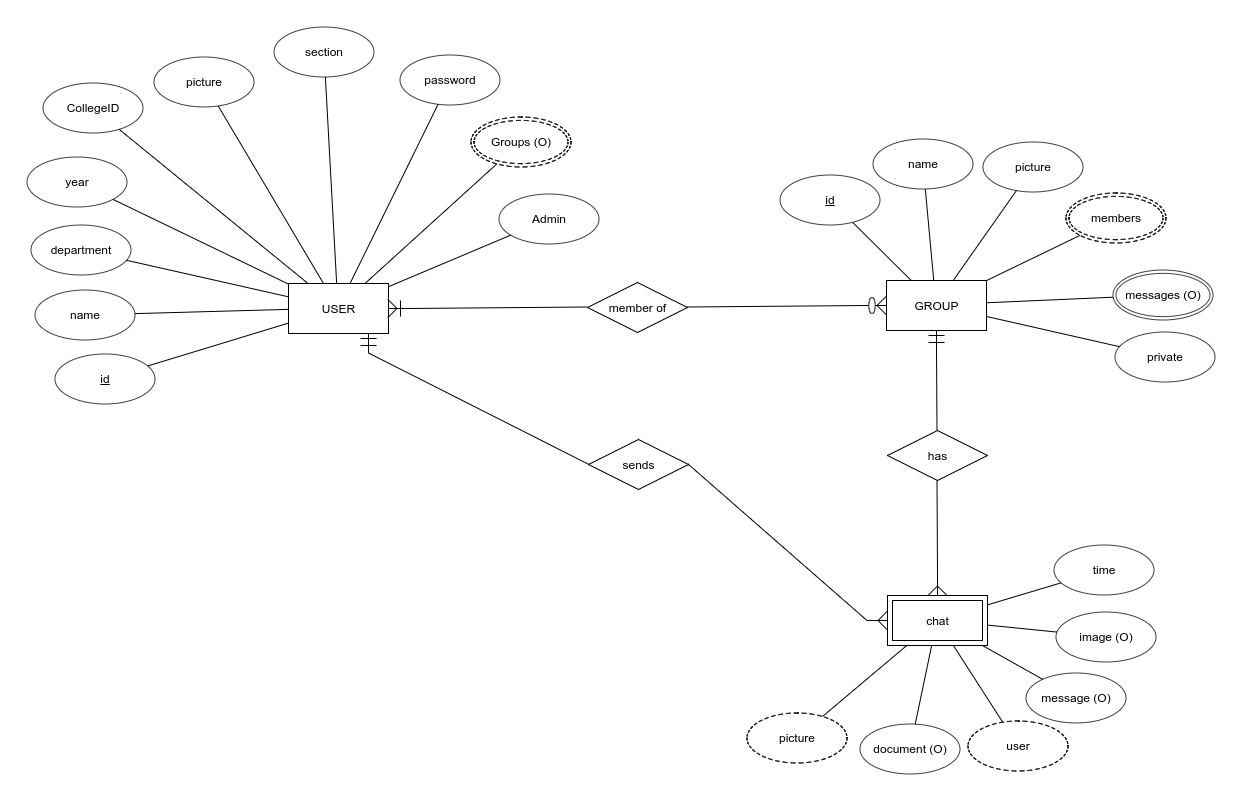
\includegraphics[scale=.4]{er2}
\end{center}

Each user can be a part of many groups and each group can contain many users, hence
the cardinality is many-to-many. Chat is the message sent in the group. A group
can have many chats(aka messages) but a chat can only belong to a group. Hence
one-to-many relation exists. Similarly, a message can be sent only by one user
whereas a user can send many messages, hence one-to-many relation exist. \\

The admin user is differentiated from the standard user using the "admin"
attribute of the user entity, which as a boolean entity. \\

The private chats are considered as two member groups by the internal structure
since they both have a similar schema. \\

\begin{center}
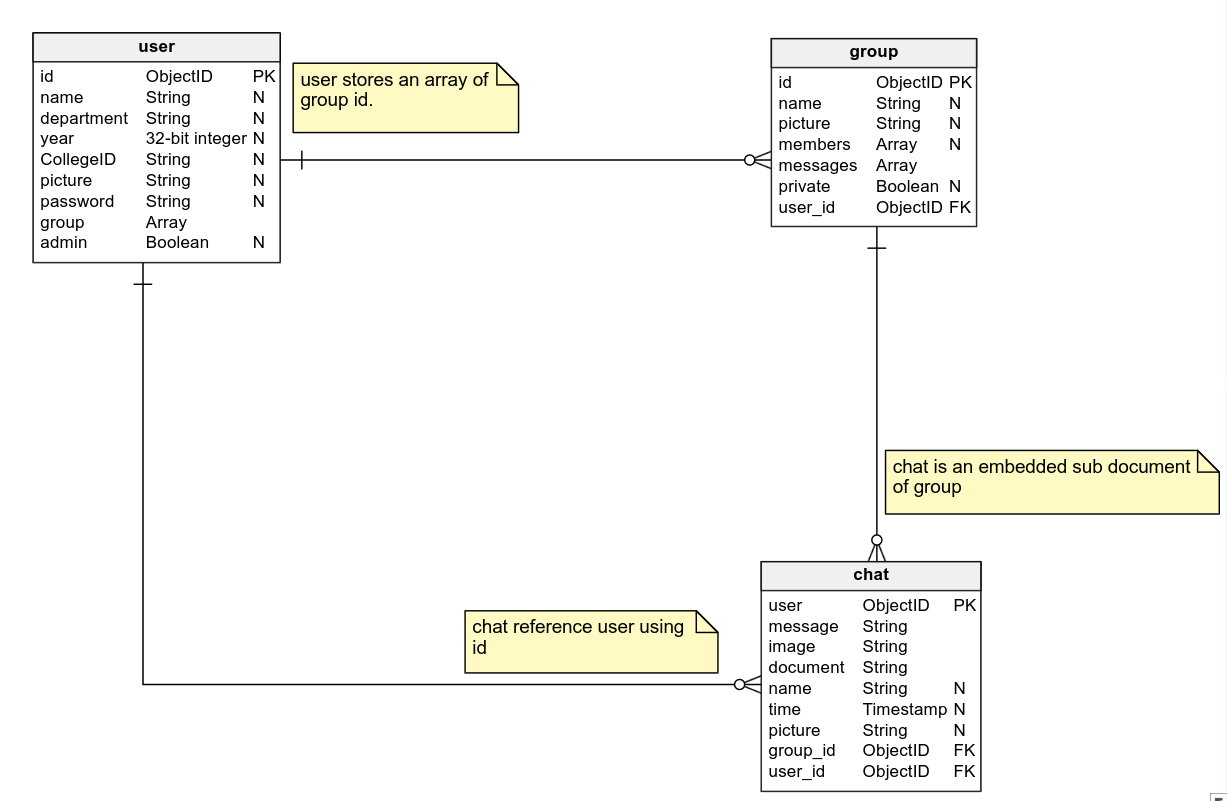
\includegraphics[scale=.4]{classdiagram}
\end{center}

The above is the schema diagram for the application's models. The user and the
group schema have a referenced relationship which means the user has an array of
group id which he is a part of and the group has an array of user id for who are
present in it. Similarly, chat has the id of the user document. Here, the chat
stores name and picture link of the user redundantly, so we don't have to query
the database twice.

\begin{center}
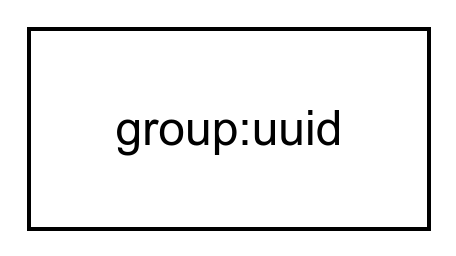
\includegraphics[scale=.4]{rediser}
\end{center}

The above schema represents the format in which the chat is stored in Redis.
Redis is an in-memory data structure store. It stores data as key-value pairs
and provides internal data structures. Here, we cache the messages as lists. The
name of the list is in the format: 'group: $\langle$ group's uuid $\rangle$ '.

%{\let\clearpage\relax \chapter{Design}}
\chapter{Design}

\section{Technology Stack}
\begin{itemize}
  \item Since we are building a real-time chat application, we need the messages to
  transmit instantaneously. So, we need the application to be asynchronous.
  Hence, we use Node.js which it is built to be asynchronous in nature.

  \item We use it with the Express.js since it is a light-weight unopinionated
  framework and hence allows us to build a light weight application which is
  best suited for this application since scalability is not an important aspect
  since it is meant to be used within the college's LAN.

  \item We use MongoDB to store the data since it is schemaless and hence allow
  us to quickly prototype the application. Moreover, light relations like the
  relation between chat(aka message) and the group can be reduced as embedded
  sub-documents an hence reducing the reducing the querying time.

  \item Since MongoDB is schemaless, we use mongoose ODM which allows us to
  design the schema at the application level and treat documents as objects.

  \item We use Redis to cache the messages and store it until a threshold of 50
  messages is reached then move it to the database. This greatly improves
  performance since  the number of database writes is reduced and moreover, the
  user can retrieve the instant past messages quickly since Redis is an in-memory
  data store.

  \item Socket.io is used to establish the web socket connection between the
  client and the server since it provides a high-level API to use web sockets
  and fall back to long polling in legacy browsers.

  \item We use Twemoji, which is twitter's emoji library which allows us to
  parse unicode to image tag to maintain consistency.

  \item Passport.js is used to create the authentication system.

  \item bcrypt is used to hash the passwords before storing.

  \item Morgan is used for logging.

  \item Gulp is used to build automation process.

  \item The frontend is built using Typescript and Angular 2 since this is a
  single page application and Angular 2 provide a clean component based separation
  for the interface.

  \item SASS 3(SCSS) is used to style the frontend since it is a superset of CSS
  and provide additional features which enable us to be more productive.

   \item Bootstrap is used to design a responsive interface quickly.

   \item Normalize.css is used to make the interface consistent throughout
   different browsers.

\end{itemize}

Therefore,
  \begin{itemize}
    \item Backend
      \begin{itemize}
        \item Node.js
        \item Express.js
        \item MongoDB with Mongoose ODM
        \item Redis
        \item Socket.io
        \item Passport.js
        \item bcrypt
        \item Morgan
        \item Gulp
      \end{itemize}

    \item Frontend
      \begin{itemize}
      \item Angular 2 with TypeScript
      \item SCSS
      \item Normalize.css
      \item Bootstrap
      \end{itemize}
  \end{itemize}

\section{User Interfaces}
When a user opens the client side with their browser, the login page appears.
In this interface, the user can enter their register number and password
to enter to the chat application.

\begin{center}
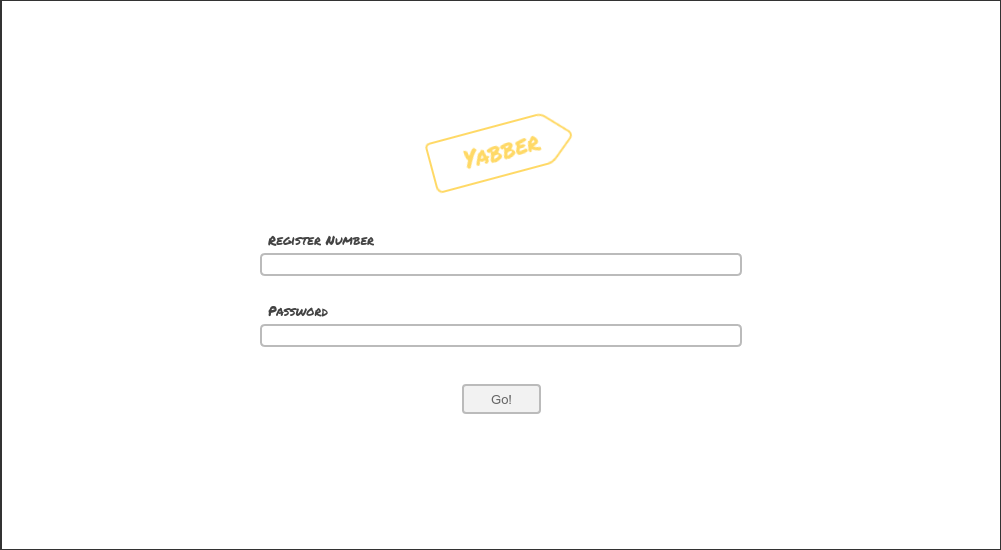
\includegraphics[scale=.29]{login}
\end{center}

The next interface on the client side would be the chat interface. Here, the
user can create groups, select group / other user and chat with them. When the
user clicks on the list item on the left side menu, the chat column on the right
side is updated with that chat's controls. The user can send emojis using the smiley
icon left of the input box and upload images and other document using either the
hamburger menu on the top right or by using the right-click context menu.

\begin{center}
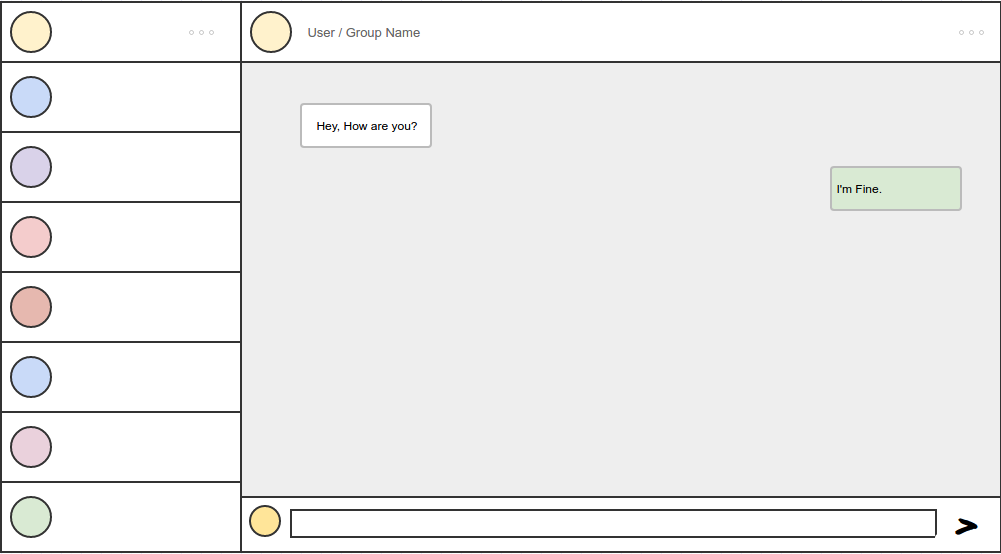
\includegraphics[scale=.3]{chat}
\end{center}

The admin panel consists of an Admin login interface using which the college
management can login into the admin panel.

\begin{center}
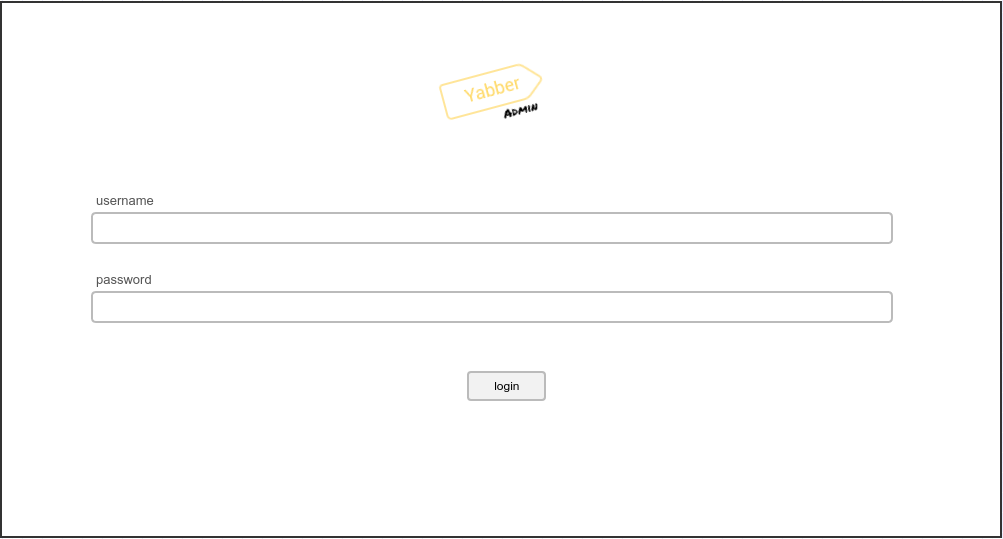
\includegraphics[scale=.3]{adminlogin}
\end{center}

The logged in admin user can add a new student using the green plus button on
the top right side and remove a student using the red minus sign next to the
student's name. The admin can modify details about the student by double clicking
the student's listing.

\begin{center}
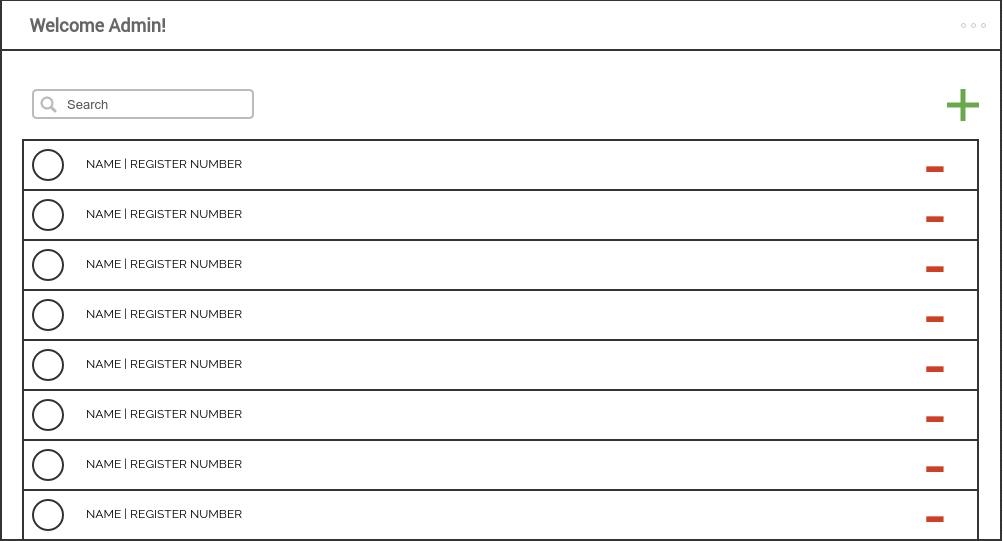
\includegraphics[scale=.3]{admin}
\end{center}

\section{Interaction Diagram}
Since Yabber is a real-time chat application, the chat process can be clearly
explained using sequence diagram. The below is the sequence diagram of the
messaging process. The first set represents user sending message and the second
set represent user receiving the message.

\begin{center}
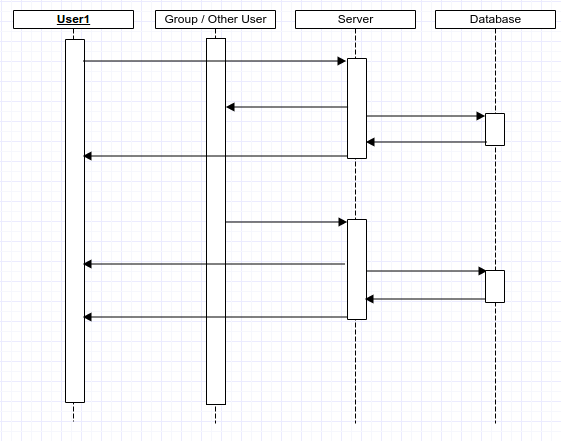
\includegraphics[scale=.8]{sequence}
\end{center}

\end{document}
